\documentclass[a6paper]{article}
\usepackage[top=0.4cm, bottom=0.25cm, left=0.25cm, right=0.25cm]{geometry}
\usepackage{tikz}
\usetikzlibrary{patterns}
\usetikzlibrary{shapes,arrows}
\usetikzlibrary{decorations.pathreplacing, positioning}

\begin{document}
\noindent
  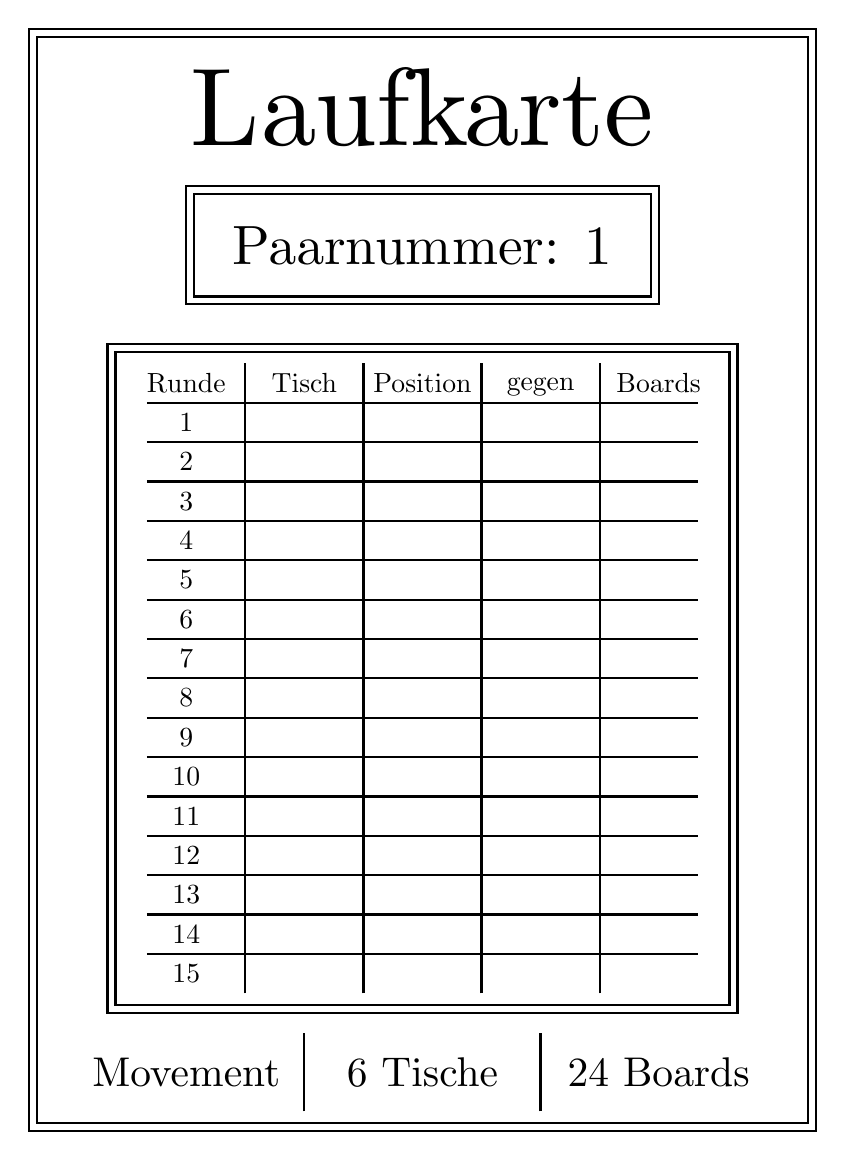
\begin{tikzpicture}

    % Border outer
    \draw[thick] (0cm,0cm) rectangle (10cm,14cm);
    \draw[thick] (0.1cm,0.1cm) rectangle (9.9cm,13.9cm);

    % Heading
    \node[very thick, scale=4] at (5cm, 13cm) {Laufkarte};

    \draw[thick] (2cm,10.5cm) rectangle (8cm,12cm);
    \draw[thick] (2.1cm,10.6cm) rectangle (7.9cm,11.9cm);
    \node[very thick, scale=2] at (5cm, 11.25cm) {Paarnummer: 1};


    % Border inner
    \draw[thick] (1cm,1.5cm) rectangle (9cm,10cm);
    \draw[thick] (1.1cm,1.6cm) rectangle (8.9cm,9.9cm);


    % Content
    \foreach [evaluate=\x as \y using 9.25 - 0.5*\x] \x in {0,...,14}
      \draw[thick] (1.5cm, \y cm) -- (8.5cm, \y cm);

    \node[very thick] at (2cm, 9.5cm) {Runde};
    \node[very thick] at (3.5cm, 9.5cm) {Tisch};
    \node[very thick] at (5cm, 9.5cm) {Position};
    \node[very thick] at (6.5cm, 9.45cm) {gegen};
    \node[very thick] at (8cm, 9.5cm) {Boards};

    \foreach [evaluate=\x as \y using 2.75 + 1.5*\x] \x in {0,...,3}
      \draw[thick] (\y cm, 1.75cm) -- (\y cm, 9.75cm);


    % Rounds
    \foreach [evaluate=\x as \y using 9.5 - 0.5*\x] \x in {1,...,15}
      \node[very thick] at (2cm, \y cm) {\x};


    % Info
    \node[very thick, scale=1.5] at (2cm, 0.75cm) {Movement};
    \draw[thick] (3.5cm, 0.25cm) -- (3.5cm, 1.25cm);

    \node[very thick, scale=1.5] at (5cm, 0.75cm) {6 Tische};
    \draw[thick] (6.5cm, 0.25cm) -- (6.5cm, 1.25cm);

    \node[very thick, scale=1.5] at (8cm, 0.75cm) {24 Boards};

    \end{tikzpicture}%
\end{document}
